\chapter{\uppercase{Implementation}}
\label{chap4}

\section{\uppercase{Implementation Environment}}
The kernel is implemented in Python using asynchronous services. The backend is FastAPI-based and the frontend is implemented with Next.js and TypeScript. Redis provides task/event channels and scheduler metadata; MongoDB stores task records and event history; ChromaDB provides persistent vector collections for planning and context swap. Provider-specific LLM usage is treated as optional metadata because some providers do not return reliable token counts.

\section{\uppercase{Semantic Agent Retrieval}}
Agent descriptions are embedded in a persistent ChromaDB collection. A task description is used as a query, and the top candidate records are returned with their distances and metadata. In the configured cosine space, ChromaDB returns $d=1-\cos(\theta)$, so the implementation reports $s=1-d$. It does not divide by two; that transformation would be appropriate for a different distance normalisation. An LRU cache reduces repeated retrieval for identical descriptions. Algorithm~\ref{alg:semantic-agent-retrieval} summarises this candidate-retrieval and cosine-distance conversion procedure.

\begin{algorithm}[H]
\caption{Semantic Agent Retrieval}
\label{alg:semantic-agent-retrieval}
\begin{algorithmic}[1]
\Require task description $q$, agent collection $C$, result count $k$
\State $r \gets C.\mathrm{query}(q,k)$
\ForAll{candidate distances $d_i$ in $r$}
\State $s_i \gets 1-d_i$
\State attach $(agent_i,s_i,description_i)$ to candidate
\EndFor
\State sort candidates by $s_i$ descending
\State \Return top candidates
\end{algorithmic}
\end{algorithm}

\section{\uppercase{Planner and Fallback}}
The planner asks the configured LLM for a structured execution plan. The response is parsed into steps and normalised against the agent registry. If the LLM request fails, exceeds quota, or produces invalid structure, a deterministic fallback creates a usable plan from the best retrieved agent(s). This maintains task execution and observability without pretending that the fallback has the same reasoning quality as the provider.

Figure~\ref{fig:optimized-planner} illustrates the complete optimized planning path, from semantic candidate retrieval through structured plan validation, fallback routing, DAG construction, scheduling, and runtime execution.
\begin{figure}[H]
\centering
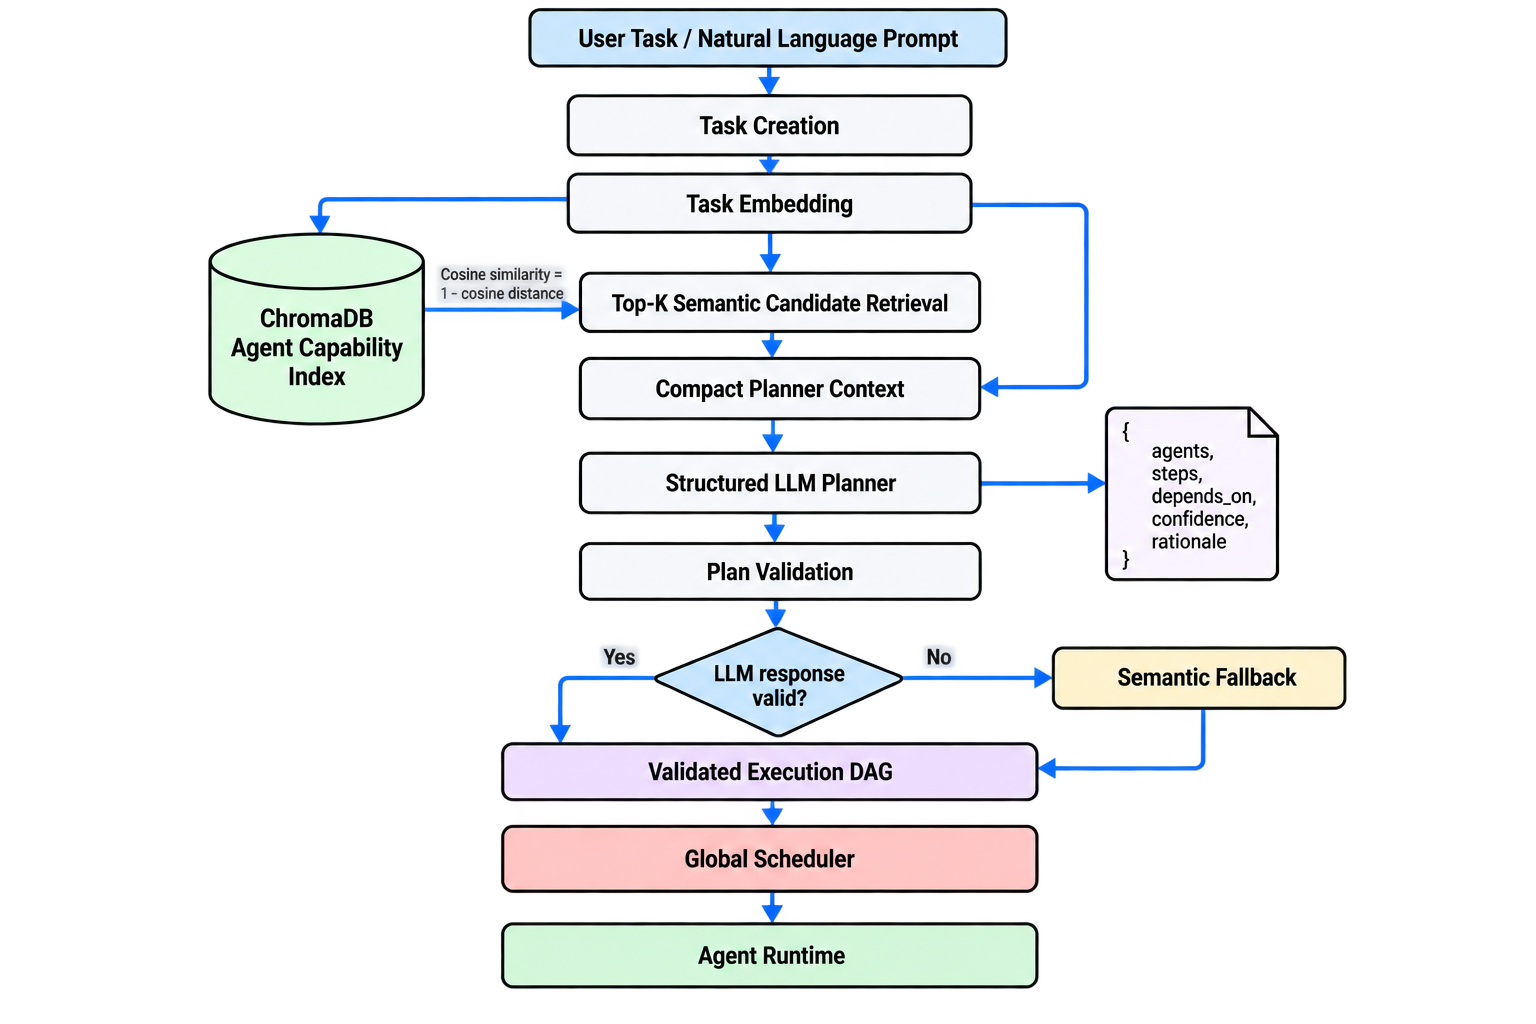
\includegraphics[width=0.98\textwidth]{4/figures/optimized_planner.png}
\caption{Optimized semantic planner and DAG construction}
\label{fig:optimized-planner}
\end{figure}

\section{\uppercase{DAG Validation}}
Every step has a unique identifier and a list of prerequisite identifiers. Validation rejects duplicate identifiers, unknown agents, unknown dependencies, and cycles. A Kahn-style topological pass counts nodes removed from the ready set. If the count is smaller than the number of steps, the dependency graph contains a cycle and is rejected. The same validated dependency lists are used to generate Mermaid edges. Algorithm~\ref{alg:dependency-validation} specifies the cycle-detection procedure.

\begin{algorithm}[H]
\caption{Dependency Validation by Cycle Detection}
\label{alg:dependency-validation}
\begin{algorithmic}[1]
\Require step set $S$
\State build adjacency list and indegree for every step
\State $Q \gets$ all steps with indegree zero
\State $visited \gets 0$
\While{$Q$ is not empty}
\State remove a step $u$ from $Q$; $visited \gets visited+1$
\ForAll{successors $v$ of $u$}
\State decrement indegree$(v)$
\If{indegree$(v)=0$} add $v$ to $Q$ \EndIf
\EndFor
\EndWhile
\If{$visited \ne |S|$} \Return invalid cyclic plan \Else \Return valid plan \EndIf
\end{algorithmic}
\end{algorithm}

\section{\uppercase{Priority-Aging Scheduler}}
The scheduler stores ready records in a Redis sorted set and keeps execution metadata in hashes. The selection score is conceptually computed as:
\begin{equation}
P_{effective}=\min(P_{base}+\alpha W,P_{max}),
\label{eq:priority}
\end{equation}
where $W$ is queue waiting time. The implementation uses an in-process pending set for dispatch coordination and persists the record so that ready and waiting work is visible and recoverable. A selected record is marked RUNNING, dispatched once, and then completed, requeued, or failed according to the result. Algorithm~\ref{alg:priority-aging-scheduler} gives the corresponding cooperative scheduling procedure.

\begin{algorithm}[H]
\caption{Global Priority-Aging Cooperative Scheduler}
\label{alg:priority-aging-scheduler}
\begin{algorithmic}[1]
\While{scheduler is active}
\State receive and persist READY records
\If{ready queue is empty} wait for event; continue \EndIf
\ForAll{ready records $a_i$} calculate $P_{effective,i}$ using Equation~\ref{eq:priority} \EndFor
\State $a^* \gets \arg\max P_{effective,i}$
\If{resource manager denies $a^*$ temporarily} mark WAITING and requeue
\ElsIf{resource manager denies permanently} mark FAILED and publish event
\Else dispatch $a^*$ cooperatively and publish RUNNING
\If{execution completes} publish COMPLETED
\ElsIf{execution waits or is requeued} publish WAITING or PREEMPTED
\Else publish FAILED
\EndIf
\EndIf
\State release resource reservations and record metrics
\EndWhile
\end{algorithmic}
\end{algorithm}

\section{\uppercase{Resource Admission and Token Budgets}}
The resource manager checks active global slots, active slots for the task, and the cumulative estimated token reservation for the task. A temporary denial leaves work waiting; an exhausted task budget is converted into a blocked/failed outcome rather than leaving the task silently pending. Actual provider usage, when available, is recorded separately from estimated admission tokens. This distinction explains why a provider such as Groq may display zero usage metadata even while the scheduler correctly enforces its configured estimate.

\section{\uppercase{Redis Events and Backend Forwarding}}
Events are JSON records containing task identifier, step identifier, agent name, execution identifier, status, timestamp, priority, effective priority, queue wait, and attempt. The kernel publishes them on \texttt{kernel\_events}; the backend subscribes and forwards them over WebSocket. Scheduler records use keys such as \texttt{agentos:scheduler:ready} and \texttt{agentos:scheduler:job:<execution\_id>}. MongoDB persists task history and event records for later inspection.
Table~\ref{tab:rediskeys} summarises the Redis channels and scheduler keys used for task transport, lifecycle events, queue persistence, and recovery.

\begin{table}[H]
\centering
\caption{Principal Redis channels and keys}
\label{tab:rediskeys}
\begin{tabularx}{\textwidth}{>{\raggedright\arraybackslash}p{0.29\textwidth}>{\raggedright\arraybackslash}X>{\raggedright\arraybackslash}p{0.29\textwidth}}
\toprule
Name & Purpose & Durability role \\
\midrule
\texttt{backend\_tasks} & New task/submission messages & Transport \\
\texttt{kernel\_events} & Lifecycle, scheduler, and execution events & Transport plus Mongo persistence \\
\texttt{agentos:\allowbreak scheduler:\allowbreak ready} & Ready queue sorted-set metadata & Recovery aid \\
\texttt{agentos:\allowbreak scheduler:\allowbreak job:\allowbreak <id>} & Per-execution state hash & Recovery aid \\
\texttt{agentos:\allowbreak task:\allowbreak <id>} & Task-level scheduler state & Inspection/recovery \\
\bottomrule
\end{tabularx}
\end{table}

\section{\uppercase{Context Page-Out and Page-In}}
The pager moves messages from the active conversation state to a persistent ChromaDB collection after a configured window is exceeded. Each page stores message content, task metadata, and an embedding. On a later turn, the current query is embedded and the collection is searched; selected messages are reintroduced in relevance order. The implementation emits page-out and page-in metrics, allowing the UI or logs to verify that paging occurred.

\clearpage
\section{\uppercase{Sandboxed Execution and Self-Healing}}
The code runner creates a scoped temporary script, launches it with \texttt{asyncio.create\_subprocess\_exec}, captures stdout/stderr, and terminates the subprocess after a strict timeout. Output size is limited to prevent unbounded memory use. On a traceback, the error is supplied to the coder/tester agent and a revised script is attempted, up to three times. The runner publishes line-oriented output and final status as kernel events. No claim is made that an ordinary subprocess is equivalent to a container or microVM security boundary.

\section{\uppercase{Frontend Observability}}
The task activity panel displays lifecycle events, scheduler state, queue position, effective priority, waiting time, attempt number, resource decisions, and token totals when provider metadata is present. The plan graph modal displays the structured graph and Mermaid source. Token fields distinguish input, output, total, and configured budget; when the provider omits usage, the interface reports that the metadata is unavailable rather than inventing a count.

\section{\uppercase{Configuration and Verification}}
Table~\ref{tab:config} lists the important policy values. Verification for this phase consists of Python compilation, TypeScript type checking, scheduler/resource smoke tests, DAG validation checks, and manual event/graph inspection. No throughput, latency, or model-quality benchmark is claimed because a controlled benchmark dataset and repeated measurement harness are not yet part of the repository.
\begin{table}[H]
\centering
\caption{Selected AgentOS configuration values}
\label{tab:config}
\begin{tabular}{>{\raggedright\arraybackslash}p{5cm}p{3cm}p{5.5cm}}
\toprule
Configuration & Default & Role \\
\midrule
Global execution slots & 3 & Maximum simultaneously admitted jobs \\
Per-task execution slots & 2 & Fairness/isolation across tasks \\
Task token budget & 50,000 & Cumulative estimated admission limit \\
Maximum scheduler priority & configurable & Upper bound for aging \\
Context active window & configurable & Number of active messages \\
Self-healing attempts & 3 & Maximum code repair retries \\
\bottomrule
\end{tabular}
\end{table}

\section{\uppercase{AgentOS Algorithmic Specification}}
The following algorithm sheets define the AgentOS execution design. Together they specify the relationship between the planner, executor, lifecycle manager, context pager, dependency-aware DAG executor, scheduler, and priority-aging model. They complement the executable implementation described above. The sheets that describe full execution-context restoration, hard time-slice suspension, permission stores, or preemption represent planned extensions where the current implementation remains cooperative or partial.
Algorithms~\ref{alg:semantic-agent-retrieval}, \ref{alg:dependency-validation}, and \ref{alg:priority-aging-scheduler} describe the implemented retrieval, validation, and scheduler procedures. Algorithms~\ref{alg:lifecycle}, \ref{alg:vm-context-paging}, \ref{alg:execute-agent}, \ref{alg:semantic-agent-planning}, \ref{alg:execute-plan-dag}, and \ref{alg:global-priority-aging-scheduler} present the lifecycle, context-paging, cooperative execution, semantic planning, DAG, and global scheduling specifications in that order. The separate priority-aging/time-slice model previously shown as Figure 4.7 has been removed; the implemented priority equation and scheduler procedure are documented earlier in this chapter.

\begin{algorithm}[H]
\caption{Agent Lifecycle Management}
\label{alg:lifecycle}
\begin{algorithmic}[1]
\Require $agent\_id$, $agent\_type$, $task\_id$
\Ensure Managed agent runtime
\State $runtime\_store[agent\_id] = (id,type,task\_id,run\_fn,status)$
\State $status \in \{\textsc{CREATED},\textsc{RUNNING},\textsc{COMPLETED},\textsc{FAILED}\}$
\Function{CreateAgent}{$agent\_id,agent\_type,task\_id$}
    \If{$agent\_id \in runtime\_store$}
        \State \textbf{raise} ``Agent already exists''
    \EndIf
    \State $run\_fn \gets \Call{GetAgentRunFunction}{agent\_type}$
    \State $runtime\_store[agent\_id] \gets (agent\_id,agent\_type,task\_id,run\_fn,\textsc{CREATED})$
    \State \Return $runtime\_store[agent\_id]$
\EndFunction
\Function{SetAgentStatus}{$agent\_id,status$}
    \State $runtime\_store[agent\_id].status \gets status$
\EndFunction
\Function{DestroyAgent}{$agent\_id$}
    \State \Call{Delete}{runtime\_store[agent\_id]}
\EndFunction
\end{algorithmic}
\end{algorithm}

\begin{algorithm}[H]
\caption{Virtual Memory Context Paging}
\label{alg:vm-context-paging}
\begin{algorithmic}[1]
\Require $T_{id}$, query $q$, messages $M=\langle m_1,\ldots,m_N\rangle$, window $W$, threshold $\tau$, top-$K$ limit $K$, embedding function $\Phi$
\Ensure $C_{final}$, the context supplied to the LLM
\State $C_{final} \gets [\text{SystemMessage}(\text{SYSTEM\_PROMPT})]$; $P_{in} \gets \emptyset$
\If{$N > W$}
    \State $P_{overflow} \gets M[1:N-W]$
    \ForAll{$m_i \in P_{overflow}$}
        \State $page\_key \gets T_{id}\Vert\texttt{\_msg\_}\Vert i$
        \If{\textbf{not} $\Call{Exists}{page\_key}$}
            \State $v_i \gets \Phi(m_i.content)$
            \State $metadata \gets \{T_{id},m_i.role,m_i.timestamp,i\}$
            \State $\Call{VectorStore.Insert}{page\_key,v_i,m_i.content,metadata}$
            \State $\Call{EmitEvent}{\texttt{context.PAGE\_OUT},T_{id},i}$
        \EndIf
    \EndFor
    \State $M_{active} \gets M[N-W+1:N]$
\Else
    \State $M_{active} \gets M$
\EndIf
\If{$N > W$ \textbf{ and } $\operatorname{Trim}(q)\neq\emptyset$}
    \State $v_q \gets \Phi(q)$; $Candidates \gets \Call{VectorStore.Search}{T_{id},v_q,K}$
    \ForAll{$p \in Candidates$}
        \State $s(p) \gets \dfrac{v_q\cdot v_p}{\lVert v_q\rVert\lVert v_p\rVert}$
        \If{$s(p)\geq\tau$}
            \State $P_{in} \gets P_{in}\cup\{p\}$
            \State $\Call{EmitEvent}{\texttt{context.PAGE\_IN},T_{id},s(p),p.text}$
        \EndIf
    \EndFor
\EndIf
\If{$P_{in}\neq\emptyset$}
    \State $R\gets\Call{FormatPagedMemory}{P_{in}}$
    \State $C_{final}\gets C_{final}\cup\{\text{SystemMessage}(R)\}$
\EndIf
\ForAll{$m \in M_{active}$}
    \If{$m.role=\texttt{human}$}
        \State $C_{final}.\Call{Append}{\text{HumanMessage}(m.content)}$
    \ElsIf{$m.role=\texttt{ai}$}
        \State $C_{final}.\Call{Append}{\text{AIMessage}(m.content)}$
    \EndIf
\EndFor
\State \Return $C_{final}$
\end{algorithmic}
\end{algorithm}

\begin{algorithm}[H]
\caption{Cooperative Time-Sliced Agent Execution}
\label{alg:execute-agent}
\begin{algorithmic}[1]
\Require Agent $A^*$ and time quantum $T_q$
\Ensure Status in $\{\textsc{COMPLETED},\textsc{WAITING},\textsc{PREEMPTED},\textsc{FAILED}\}$
\Procedure{ExecuteAgent}{$A^*,T_q$}
    \If{$A^*.execution\_context$ exists}
        \State $runtime \gets \Call{RestoreExecutionContext}{A^*}$
    \Else
        \State $runtime \gets \Call{InitializeAgentRuntime}{A^*}$
    \EndIf
    \State $start\_time \gets \Call{GetCurrentTime}{}$; \Call{SetAgentStatus}{$A^*.id,\textsc{RUNNING}$}
    \While{\textbf{true}}
        \If{\Call{AgentExecutionFailed}{runtime}}
            \State \Call{SaveExecutionContext}{$A^*,runtime$}; \Return \textsc{FAILED}
        \EndIf
        \If{\Call{AgentIsWaiting}{runtime}}
            \State \Call{SaveExecutionContext}{$A^*,runtime$}; \Return \textsc{WAITING}
        \EndIf
        \If{$\Call{GetCurrentTime}{}-start\_time\geq T_q$}
            \State \Call{SaveExecutionContext}{$A^*,runtime$}; \Call{SuspendAgentExecution}{runtime}; \Return \textsc{PREEMPTED}
        \EndIf
        \State $result \gets \Call{ExecuteNextStep}{runtime}$
        \If{$result=\textsc{COMPLETED}$}
            \State $A^*.result \gets \Call{GetExecutionResult}{runtime}$; \Call{DestroyExecutionContext}{runtime}; \Return \textsc{COMPLETED}
        \ElsIf{$result=\textsc{WAITING}$}
            \State \Call{SaveExecutionContext}{$A^*,runtime$}; \Return \textsc{WAITING}
        \ElsIf{$result=\textsc{FAILED}$}
            \State \Call{SaveExecutionContext}{$A^*,runtime$}; \Return \textsc{FAILED}
        \EndIf
    \EndWhile
\EndProcedure
\end{algorithmic}
\end{algorithm}

\clearpage
\begin{algorithm}[H]
\caption{Semantic Dependency-Aware Agent Planning}
\label{alg:semantic-agent-planning}
\begin{algorithmic}[1]
\Require User task $q$, registry $A$, top-$K$ limit $K$, planner model $L$
\Ensure Valid execution DAG $G=(V,E)$
\If{capability index is not initialized}
    \ForAll{$a_i\in A$}
        \State $d_i\gets$ capability description; $e_i\gets\operatorname{Embed}(d_i)$; store $(a_i,d_i,e_i)$
    \EndFor
\EndIf
\State $e_q\gets\operatorname{Embed}(q)$; $C\gets\operatorname{SelectTopKAgents}(A,\operatorname{CosineSimilarity}(e_q,e_i),K)$
\State $P\gets\operatorname{BuildPlannerPrompt}(q,C)$; $R\gets\operatorname{LanguageModelGenerateJSON}(L,P)$
\If{$R$ contains valid DAG steps}
    \State $S\gets R.steps$
\Else
    \State $S\gets\operatorname{ConvertAgentListToSequentialSteps}(R.agents)$
\EndIf
\State $S\gets\operatorname{RemoveUnknownAgents}(S,A)$
\State $S\gets\operatorname{RemoveAgentsNotInCandidates}(S,C)$
\State $S\gets\operatorname{RemoveDuplicateStepIDs}(S)$; $S\gets\operatorname{RemoveInvalidDependencies}(S)$
\State $S\gets\operatorname{ValidateAcyclicity}(S)$
\If{$S$ contains a cycle}
    \State $S\gets\operatorname{ConvertAgentListToSequentialSteps}(R.agents)$
\EndIf
\State $G\gets\operatorname{BuildGraph}(S)$; $M\gets\operatorname{GenerateMermaidDiagram}(G)$
\State $\operatorname{Persist}(G,M)$; $\operatorname{EmitPlanningEvent}(G,M)$
\State \Return $G$
\end{algorithmic}
\end{algorithm}

\begin{algorithm}[H]
\caption{Dependency-Aware Agent DAG Execution}
\label{alg:execute-plan-dag}
\begin{algorithmic}[1]
\Require Execution DAG $G=(V,E)$ and task state
\Ensure Results produced by all executed agents
\State $completed\gets\emptyset$
\While{$completed\neq V$}
    \State $ready\gets\emptyset$
    \ForAll{$v\in V$}
        \If{$v\notin completed$ \textbf{ and } $\operatorname{Dependencies}(v)\subseteq completed$}
            \State $ready\gets ready\cup\{v\}$
        \EndIf
    \EndFor
    \If{$ready=\emptyset$} \State \textbf{raise} $\operatorname{InvalidPlanCycle}$ \EndIf
    \State $v\gets\operatorname{SchedulerSelect}(ready)$; $result\gets\operatorname{ExecuteAgent}(v.agent)$
    \State $\operatorname{StoreResult}(v,result)$; $completed\gets completed\cup\{v\}$
\EndWhile
\State \Return all results
\end{algorithmic}
\end{algorithm}

\begin{algorithm}[H]
\caption{Global Priority-Aging Cooperative Agent Scheduler}
\label{alg:global-priority-aging-scheduler}
\begin{algorithmic}[1]
\Require Redis ready queue $Q$, aging factor $\alpha$, maximum priority $P_{max}$, quantum $T_q$, resource manager $R$
\Ensure Scheduled agent execution
\While{AgentOS is active}
    \State Receive \texttt{AGENT\_READY} events and insert agents into $Q$
    \If{$Q=\emptyset$} \State Wait for the next scheduler event; \textbf{continue} \EndIf
    \State $t\gets\operatorname{CurrentTime}()$
    \ForAll{$A_i\in Q$}
        \State $W_i\gets t-A_i.ready\_time$; $P_i^{eff}\gets\min(P_i^{base}+\alpha W_i,P_{max})$
    \EndFor
    \State $A^*\gets\arg\max_{A_i\in Q}P_i^{eff}$; $auth\gets R.\operatorname{request}(A^*)$
    \If{$auth=\mathrm{DENIED}$}
        \If{denial is temporary} \State Mark $A^*$ WAITING and reinsert into $Q$
        \Else \State Mark $A^*$ FAILED and publish \texttt{AGENT\_FAILED} \EndIf
        \State \textbf{continue}
    \EndIf
    \State Remove $A^*$ from $Q$; mark RUNNING; publish \texttt{AGENT\_RUNNING}
    \State $r\gets\operatorname{Dispatch}(A^*,T_q)$
    \If{$r=\mathrm{COMPLETED}$} \State Mark COMPLETED; publish \texttt{AGENT\_COMPLETED}
    \ElsIf{$r=\mathrm{WAITING}$} \State Mark WAITING
    \ElsIf{$r=\mathrm{PREEMPTED}$} \State Mark READY, update $ready\_time$, reinsert into $Q$, publish \texttt{AGENT\_PREEMPTED}
    \Else \State Mark FAILED; publish \texttt{AGENT\_FAILED}
    \EndIf
    \State $\operatorname{ReleaseResources}(A^*)$; $\operatorname{RecordMetrics}(A^*,r)$
\EndWhile
\end{algorithmic}
\end{algorithm}
